\documentclass{book}

\usepackage[utf8]{inputenc}
\usepackage{titlesec}
\usepackage{easylist}
\usepackage{hanging}
\usepackage{hyperref}
\usepackage[a4paper,top=2.0cm,bottom=2.0cm,left=2.0cm,right=2.0cm]{geometry}
\usepackage{blindtext}
\usepackage{tipa}
\usepackage{epigraph}
\usepackage{enumerate}
\usepackage{longtable}
\usepackage{setspace}
\usepackage{verbatim}
\usepackage[T1]{fontenc}
\usepackage{graphicx}
\usepackage[italian]{babel}
\usepackage{amsmath}
\usepackage{pbox}
\usepackage{fancyhdr}
\usepackage{cancel}
\usepackage{tabularx}
\usepackage{booktabs}
\usepackage{multirow}
\usepackage{longtable}
\usepackage{tikz}
\usepackage{tikz-qtree}
\usepackage{subfig}
\usepackage{xcolor}
\usepackage{amssymb}
\usepackage{mathrsfs}
\usepackage{textcomp}
\usepackage{xfrac}

\usepackage{listings}
\usepackage{color}

\definecolor{mygreen}{rgb}{0,0.6,0}
\definecolor{mygray}{rgb}{0.5,0.5,0.5}
\definecolor{mymauve}{rgb}{0.58,0,0.82}

\lstset{ 
  backgroundcolor=\color{white},   % choose the background color; you must add \usepackage{color} or \usepackage{xcolor}; should come as last argument
  basicstyle=\footnotesize,        % the size of the fonts that are used for the code
  breakatwhitespace=false,         % sets if automatic breaks should only happen at whitespace
  breaklines=true,                 % sets automatic line breaking
  captionpos=b,                    % sets the caption-position to bottom
  commentstyle=\color{mygreen},    % comment style
  deletekeywords={...},            % if you want to delete keywords from the given language
  escapeinside={\%*}{*)},          % if you want to add LaTeX within your code
  extendedchars=true,              % lets you use non-ASCII characters; for 8-bits encodings only, does not work with UTF-8
  firstnumber=1000,                % start line enumeration with line 1000
  frame=single,	                   % adds a frame around the code
  keepspaces=true,                 % keeps spaces in text, useful for keeping indentation of code (possibly needs columns=flexible)
  keywordstyle=\color{blue},       % keyword style
  language=Octave,                 % the language of the code
  morekeywords={*,...},            % if you want to add more keywords to the set
  numbers=left,                    % where to put the line-numbers; possible values are (none, left, right)
  numbersep=5pt,                   % how far the line-numbers are from the code
  numberstyle=\tiny\color{mygray}, % the style that is used for the line-numbers
  rulecolor=\color{black},         % if not set, the frame-color may be changed on line-breaks within not-black text (e.g. comments (green here))
  showspaces=false,                % show spaces everywhere adding particular underscores; it overrides 'showstringspaces'
  showstringspaces=false,          % underline spaces within strings only
  showtabs=false,                  % show tabs within strings adding particular underscores
  stepnumber=2,                    % the step between two line-numbers. If it's 1, each line will be numbered
  stringstyle=\color{mymauve},     % string literal style
  tabsize=2,	                   % sets default tabsize to 2 spaces
  title=\lstname                   % show the filename of files included with \lstinputlisting; also try caption instead of title
}

\linespread{1.5} % l'interlinea

\frenchspacing

\newcommand{\abs}[1]{\lvert#1\rvert}

\usepackage{floatflt,epsfig}

\usepackage{multicol}
\newcommand\yellowbigsqcup[1][\displaystyle]{%
  \fboxrule0pt
  \ifx#1\textstyle\fboxsep-0.6pt\else\fboxsep-1.25pt\fi
  \mathrel{\fcolorbox{white}{yellow}{$#1\bigsqcup$}}}

\title{Formulario Fisica 1}
\author{Nicola Ferru}
\newtheorem{defi}{Definizione}[section]
\begin{document}
\maketitle
\chapter{Cinematica}
\label{sec:cin}

\section{Moto uniformemente accelerato}
\label{sec:motouniacc}

Formula per calcolare la Velocità finale:
\begin{equation}
  \label{eq:vf}
  V_f=v_0+a\cdot t
\end{equation}
di cui le singole variabili hanno il seguente significato:
\begin{itemize}
\item $v_0$ è la velocità di partenza;
\item $a$ è l'accelerazione;
\item $t$ è il periodo di tempo.
\end{itemize}

\subsection{Segmento percorso $s$ dopo il tempo $t$}
\label{sec:segPDTempt}
Per il parloco del segmento percorso $s$, se prendiamo come riferimento la perte dopo il tepo $t$, dobbiamo utilizzare:
\begin{equation}
  \label{eq:segperdopot}
  s=s_0+v_0\cdot t \pm \frac{a}{2}\cdot t^2
\end{equation}
Il segno dipende dal sistema di riferimento -- Le veriabili in gioco sono le seguenti:
\begin{itemize}
\item $s_0$ il segmento nel momento iniziale;
\item $v_0$ la velocità nel momento iniziale;
\item $a$ accelerazione;
\item $t$ il periodo di tempo.
\end{itemize}

\subsection{Corpo che cade}
\label{sec:corpochecade}
\begin{equation}
  \label{eq:altezzadicaduta}
  h=h_0+v_0\cdot t \pm \frac{g}{2}\cdot t^2
\end{equation}
Il segno dipende dal sistema di riferimento -- le variabili in gioco sono:
\begin{itemize}
\item $h_0$ altezza nel momento iniziale;
\item $v_0$ la velocità nel momento iniziale;
\item $t$ il periodo di tempo;
\item $g$ forza peso.
\end{itemize}

\subsection{Caduta da $h_0$ con velocità iniziale nulla}
Le formule correlate ad un grave che cade da un altezza $h_0$ con una velocità $v_0=0$, sono le seguenti:
\label{sec:cadutadahconvelzero}
\begin{multicols}{2}
  \subsubsection{Tempo di caduta}
  \label{sec:tempcad}
  \begin{equation}
    \label{eq:tempcad}
    t_c=\sqrt{\frac{2h_0}{g}}
  \end{equation}
  \subsubsection{Velocità finale}
  \label{sec:velFin}
  \begin{equation}
    \label{eq:velfin}
    V_f=\sqrt{2gh}
  \end{equation}
\end{multicols}
Visto che la velocità conosciutà è quella iniziale che è nulla, all'interno delle formule sono presenti solamente l'altezza $h_0$ e la forza peso $g$.

\subsection{Lancio verso l'alto}
\label{sec:lancioversolalto}
Nel caso del lancio verso l'alto sono presenti queste due formule:
\begin{multicols}{2}
  \subsubsection{Altezza finale}
  \label{sec:altfinlancioversalt}
  \begin{equation}
    \label{eq:altfinlancioversalt}
    h=\frac{V_0^2}{2g}
  \end{equation}
  \subsubsection{Tempo finale}
  \label{sec:tempofinlancioveralt}
  \begin{equation}
    \label{eq:tempofinlancioveralt}
    t_h=\frac{V_0}{g}
  \end{equation}
\end{multicols}
In questo caso le variabile che entrano in gioco sono:
\begin{itemize}
\item La velocità $V_0$;
\item La forza peso $g$.
\end{itemize}

\section{Moto circolare unicorme}
\label{sec:motCircUni}
\begin{defi}
  Il moto circolare uniforme è il moto di un punto che percorre una traiettoria circolare (moto circolare) con velocità costante (moto uniforme). Velocità costante vuol dire che percorre archi di uguale lunghezza in intervallo di tempo uguale. La velocità si rappresenta un vettore tangente alla circonferenza (perpendicolare al raggio), vettore che ha modulo costante ma cambia continuamente direzione. \\
  L'accelerazione tangenziale, che è dovuta alle variazioni del modulo della velocità, è quindi nulla. L'accelerazione centripeta, che è dovua alle variazioni della direzione della velocità, non è nulla ed ha modulo costante. Il verso del moto circolare si dice orario se è concorde con quello delle lancette dell'orologio, antiorario in caso contrario.
  \begin{multicols}{2}
    \subsubsection{Accelerazione centripeta}
    \label{sec:acccent}
    \begin{equation}
      \label{eq:acccentripeta}
      a_c=\frac{V^2}{r}
    \end{equation}
    \subsubsection{Velocità angolare}
    \label{sec:velang}
    \begin{equation}
      \label{eq:velang}
      \omega=\sfrac{2\pi_{rad}}{T}=2\pi\cdot v
    \end{equation}
    \begin{equation}
      \label{eq:Velang}
      \omega = \frac{\Delta \alpha}{\Delta t}
    \end{equation}
  \end{multicols}
  $\Delta\alpha =$ angolo spezzato al centro
\end{defi}

\subsection{Energia cinetica totale}
\label{sec:encintot}

\begin{equation}
  \label{eq:encintot}
  E=\frac{1}{2} mv^2
\end{equation}

\subsection{Forza centripeta e centrifuga}
\label{sec:forzcentecentr}

\begin{multicols}{2}
  \subsubsection{Forza centripeta}
  \label{sec:forzacent}
  \begin{equation}
    \label{eq:forzacent}
    F_{CP}=m\cdot \frac{v^2}{r}
  \end{equation}
  
  \subsubsection{Forza centrifuga}
  \label{sec:forzacentrifuga}
  \begin{equation}
    \label{eq:forzacentrifuga}
    F_{CF}=-m\cdot\frac{v^2}{r}
  \end{equation}
\end{multicols}
Dato che le due formule danno due valori uno opposto all'altro possiamo dire senza ombra di dubbio che:
\begin{equation}
  \label{eq:equalscrcrnt}
  \boxed{F_{CP}=-F_{CF}}
\end{equation}
\begin{defi}
  Ogni lato di un triangolo rettangolo è maggiore della differenza degli altri due e minore della loro somma.
\end{defi}

\section{Somma dei vettori}
\label{sec:sommavect}
La somma dei vettori segue il seguente cruterio:
\begin{equation}
  \label{eq:sommavect}
  \abs{\vec{v}}=\sqrt{\abs{v_1}^2+\abs{v_2}^2+2\abs{v_1}\abs{v_2}+\log \alpha}
\end{equation}
La posizione e direzione di un vettore sono fondamentali per capire come essi agiscano. I tre casi più comuni sono:
\begin{description}
\item[Ortogonali] $\abs{v}=\sqrt{\abs{v_1}^2+\abs{v_2}^2}$
\item[Stessa direzione, vorso concorde] $\abs{v}=\abs{v_1}+\abs{v_2}$
\item[Stessa direzione, verso opposto] $\abs{v}=\abs{v_1}-\abs{v_2}$
\end{description}

\section{Prodotto tra vettori}
\label{sec:prodottotravect}

\subsection{Scalare}
\label{sec:scalare}

\begin{equation}
  \label{eq:scalare}
  a\cdot b=a\cdot\abs{b_p}
\end{equation}
Di cui $\abs{b_p}$ è il componente di $b//ad\text{ }a$
\begin{figure}[ht!]
  \centering
  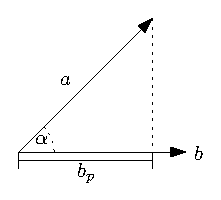
\includegraphics{img/scalare.eps}
  \caption{prodotto vettoriale scalare}
  \label{fig:prodvectscal}
\end{figure}
\begin{equation}
  \label{eq:scalare2}
  a\cdot b= a\cdot b\cdot \cos \alpha
\end{equation}

\subsection{Vettoriale}
\label{sec:vectprod}
\begin{equation}
  \label{eq:prodvec}
  \begin{matrix}
    a\cdot b=a\cdot b\cdot \sin \alpha & a_n \dot b
  \end{matrix}
\end{equation}
di cui, $a_n$ è componente di $a \bot a b$.

\end{document}
